\documentclass[12pt,a4paper,french]{report}

% =========================================================
% PACKAGES
% =========================================================

\usepackage[french]{babel}

\usepackage{fontspec}
\setmainfont{Times New Roman}

\usepackage{graphicx}
\usepackage{geometry}
\usepackage{setspace}
\usepackage{array}
\usepackage{booktabs}
\usepackage{float}
\usepackage{ragged2e}

\usepackage{tocloft}
\renewcommand{\cftchapleader}{\cftdotfill{\cftdotsep}}  % dots
\renewcommand{\cftchapafterpnum}{\cftparfillskip}
\renewcommand{\cftchapfont}{\bfseries}
\renewcommand{\cftchappagefont}{\bfseries}

\usepackage{fancyhdr}

\usepackage[hidelinks,hypertexnames=false]{hyperref}   % always last
% =========================================================
% PAGE SETTINGS
% =========================================================

\geometry{
    top=2cm,
    bottom=2cm,
    left=2cm,
    right=2cm
}

\onehalfspacing
\justifying
\hyphenpenalty=10000
\exhyphenpenalty=10000
\emergencystretch=3em
\sloppy


% =========================================================
% HEADER AND FOOTER
% =========================================================

\pagestyle{fancy}

\fancyhf{} % Clear default header/footer

% Header: chapter number and title on the right
\fancyhead[R]{\nouppercase{\leftmark}}

% Footer: page number centered
\fancyfoot[C]{\thepage}

% Header line
\renewcommand{\headrulewidth}{0.4pt}

% Footer line
\renewcommand{\footrulewidth}{0pt}

% Chapter opening pages: no header
\fancypagestyle{plain}{
    \fancyhf{}
    \fancyfoot[C]{\thepage}
    \renewcommand{\headrulewidth}{0pt}
}

% =========================================================
% TABLE OF CONTENTS SETTINGS
% =========================================================

\setcounter{tocdepth}{3}
\setcounter{secnumdepth}{3}


% =========================================================
% DOCUMENT
% =========================================================

\begin{document}
% =========================================================
% COVER PAGE
% =========================================================

\begin{titlepage}
    \centering

    % Institutional header
    {\small \textbf{MINISTÈRE DE L'ENSEIGNEMENT SUPÉRIEUR ET DE LA}}\\
    {\small \textbf{RECHERCHE SCIENTIFIQUE}}\\[0.15cm]

    {\small \textbf{UNIVERSITÉ DE SOUSSE}}\\[0.15cm]

    {\small \textbf{INSTITUT SUPÉRIEUR D'INFORMATIQUE}}\\
    {\small \textbf{ET DES TECHNOLOGIES DE COMMUNICATION}}\\[0.7cm]

    % Logo
    
\includegraphics[width=0.20\textwidth]{figures/logo-isitcom.png}\\[0.7cm]

    % Report type
    {\large \textbf{Rapport de mini-projet}}\\[0.25cm]

    {\normalsize
    Spécialité : Systèmes Embarqués et Internet des Objets
    }\\[0.8cm]

    % Project title
    {\LARGE \textbf{PET-Recycling-Filament-System}}\\[0.25cm]

    {\normalsize
    \textit{Système IoT pour le Recyclage du PET}
    }\\[1.0cm]

    % Author
    {\normalsize Réalisé par :}\\[0.15cm]
    {\normalsize \textbf{Anouer Chouikh}}\\[0.7cm]

    % Supervisor
    {\normalsize Encadré par :}\\[0.15cm]
    {\normalsize \textbf{Melek Chouchene}}\\[1.0cm]

    % Horizontal line
    \rule{0.75\textwidth}{0.5pt}\\[0.4cm]

    % Academic year
    {\normalsize \textbf{Année universitaire 2026/2027}}\\[0.8cm]

    % Footer
    {\small
    Institut Supérieur d'Informatique et des Technologies de Communication\\
    Tél/Fax : +216 73 37 15 71 / +216 73 38 44 11
    }

\end{titlepage}
\pagenumbering{roman}



% =========================================================
% ACKNOWLEDGEMENTS
% =========================================================

\chapter*{Remerciements}

Nous remercions toutes les personnes qui ont contribué, directement ou
indirectement, à la réalisation de ce projet.

Nous exprimons particulièrement notre gratitude à notre encadrant pour
son accompagnement, ses conseils et ses orientations tout au long de
ce travail.

Nous remercions également l'Institut Supérieur d'Informatique et des
Technologies de Communication pour les connaissances et les ressources
mises à notre disposition.

% =========================================================
% TABLE OF CONTENTS
% =========================================================
\newpage


\tableofcontents

\newpage
\listoffigures


% =========================================================
% CHAPTER 1
% =========================================================

\chapter{Description du Projet}
\pagenumbering{arabic}

% =========================================================
% CHAPITRE 1 — DESCRIPTION DU PROJET
% =========================================================

\section{Introduction}

Le développement durable et la réduction des déchets plastiques constituent
aujourd'hui des enjeux importants sur les plans environnemental, économique
et technologique. Parmi les matières plastiques les plus utilisées, le
polyéthylène téréphtalate (PET) occupe une place importante, notamment dans
la fabrication des bouteilles et des emballages.

Le PET présente cependant l'avantage d'être recyclable et peut être valorisé
afin de produire de nouveaux matériaux. Dans le domaine de la fabrication
additive, le plastique recyclé peut notamment être transformé en filament
destiné à l'impression 3D. Cette approche permet de donner une seconde vie
aux déchets plastiques tout en réduisant la consommation de matière première.

C'est dans ce contexte que s'inscrit le projet \textit{3awedlou}, une
solution IoT dédiée au recyclage du PET et à sa transformation en filament
pour impression 3D. Le projet associe une partie matérielle permettant les
différentes étapes du processus de transformation à une architecture
logicielle destinée à la supervision et au suivi des données de la machine.

L'objectif de ce projet ne se limite donc pas à la réalisation d'une
machine de transformation du plastique. Il vise également à intégrer les
principes de l'Internet des Objets afin de rendre le système connecté,
supervisable et capable de fournir des informations sur son fonctionnement.

\section{Problématique}

La gestion des déchets plastiques représente un défi important en raison de
leur volume, de leur durée de dégradation et de leur utilisation massive
dans de nombreux secteurs. Le PET, largement présent dans les bouteilles
plastiques, constitue une matière particulièrement intéressante pour la
valorisation en raison de ses propriétés et de sa recyclabilité.

Cependant, transformer des déchets plastiques en un matériau utilisable
pour l'impression 3D nécessite plusieurs opérations successives. Le
plastique doit notamment être préparé, chauffé, fondu et extrudé de manière
contrôlée afin d'obtenir un filament présentant des caractéristiques
adaptées à son utilisation.

Une difficulté supplémentaire réside dans le contrôle et la supervision de
ces différentes opérations. La température, le fonctionnement du moteur,
l'état de la machine et les paramètres de production doivent pouvoir être
surveillés afin d'améliorer la fiabilité du système et d'identifier
rapidement les éventuels problèmes.

La problématique principale de ce projet peut ainsi être formulée comme
suit :

\begin{quote}
\textit{Comment concevoir et réaliser une machine connectée capable de
transformer des déchets PET en filament pour impression 3D tout en
permettant le contrôle, la supervision et la collecte des données de son
fonctionnement ?}
\end{quote}

Cette problématique implique donc à la fois des considérations mécaniques,
électroniques, informatiques et liées à l'Internet des Objets.

\section{Solution Proposée}

Afin de répondre à cette problématique, le projet propose la conception et
la réalisation d'un système de recyclage du PET intégrant une architecture
IoT.

La solution repose sur une machine physique chargée d'assurer la
transformation du plastique. La partie matérielle comprend notamment un
système de chauffage et de contrôle de température, un moteur pas à pas
destiné à l'extrusion du matériau ainsi que différents éléments
électroniques permettant le pilotage et la mesure des paramètres de
fonctionnement.

La commande du système est assurée par un microcontrôleur Arduino Mega.
Celui-ci prend en charge une partie du contrôle local de la machine,
notamment la gestion du moteur et du système de chauffage. Un ESP32 est
également intégré à l'architecture afin d'assurer les fonctions de
communication et de connectivité du système.

La communication entre les différents éléments permet de séparer les
fonctions de contrôle temps réel de la machine et les fonctions de
communication avec les services logiciels. Cette architecture facilite
ainsi l'évolution du système et son intégration dans une infrastructure
IoT.

Sur le plan logiciel, le système est associé à une application permettant
de superviser la machine et d'exploiter les données collectées. Le backend
constitue l'intermédiaire entre les équipements connectés et les
applications clientes. Il permet notamment de gérer les utilisateurs, les
machines, les sessions de fonctionnement, les données de télémétrie et les
informations relatives à la production.

La communication IoT est basée sur le protocole MQTT, particulièrement
adapté aux systèmes connectés grâce à son modèle de communication
publish/subscribe et à sa faible surcharge. Les données provenant de la
machine peuvent ainsi être transmises au backend afin d'être enregistrées
et exploitées par les interfaces de supervision.

L'architecture globale du système peut être représentée selon plusieurs
niveaux : la machine et ses capteurs/actionneurs constituent la couche
physique, les microcontrôleurs assurent le contrôle et la communication,
le backend assure la gestion des données et les applications web et
mobiles permettent leur visualisation et leur exploitation.

Cette approche permet de transformer une machine de recyclage classique en
un système connecté capable de fournir des informations en temps réel sur
son fonctionnement. Elle constitue également une base évolutive pour
l'ajout de nouvelles fonctionnalités telles que l'analyse des données,
l'amélioration du contrôle du processus ou encore la maintenance
préventive.

\section{Conclusion}

Dans ce chapitre, nous avons présenté le contexte général du projet
\textit{3awedlou}, ainsi que la problématique liée à la valorisation des
déchets PET et à leur transformation en filament pour impression 3D.

La solution proposée repose sur l'association d'une machine de recyclage,
de systèmes embarqués et d'une architecture IoT permettant le contrôle, la
communication et la supervision du système.

Après avoir présenté le projet et ses objectifs généraux, le chapitre
suivant sera consacré à l'étude détaillée des besoins ainsi qu'à la
conception matérielle et logicielle de la solution.


% =========================================================
% CHAPTER 2
% =========================================================

\chapter{Conception et Étude des Besoins}

% =========================================================
% CHAPITRE 2 — CONCEPTION ET ÉTUDE DES BESOINS
% =========================================================

\section{Introduction}

Après avoir présenté le contexte général du projet, sa problématique et la
solution proposée, ce chapitre est consacré à l'étude des besoins et à la
conception du système \textit{3awedlou}.

L'objectif de cette étape est de définir les fonctionnalités attendues,
les contraintes auxquelles le système doit répondre ainsi que
l'architecture générale permettant d'assurer la communication entre la
machine, les systèmes embarqués, le serveur et les applications clientes.

La conception est organisée autour de plusieurs aspects complémentaires :
l'analyse des besoins fonctionnels et non fonctionnels, l'étude de
l'enchaînement des données, la définition de l'architecture matérielle et
logicielle, l'étude des protocoles de communication IoT ainsi que la
modélisation UML du système.

\section{Besoins fonctionnels}

Les besoins fonctionnels décrivent les services et les fonctionnalités que
le système doit fournir à ses différents utilisateurs et composants.

Dans le cadre du projet \textit{3awedlou}, les principales fonctionnalités
identifiées sont les suivantes.

\subsection{Gestion des utilisateurs}

Le système doit permettre aux utilisateurs autorisés d'accéder à
l'application et d'utiliser les fonctionnalités correspondant à leurs
droits d'accès. L'authentification permet notamment de sécuriser l'accès
aux informations relatives aux machines et aux productions.

\subsection{Gestion des machines}

L'application doit permettre de gérer les machines connectées au système.
Pour chaque machine, les informations relatives à son identification et à
son état doivent être accessibles.

Le système doit notamment permettre de connaître l'état courant d'une
machine, par exemple :

\begin{itemize}
    \item en attente ;
    \item en cours de chauffage ;
    \item en extrusion ;
    \item en pause ;
    \item en erreur ;
    \item hors ligne.
\end{itemize}

\subsection{Acquisition des données}

La machine doit être capable de mesurer et de transmettre différentes
données relatives à son fonctionnement. Ces données peuvent notamment
concerner la température, l'état du moteur, l'état général de la machine
et les informations relatives à une session de production.

\subsection{Supervision de la machine}

Le système doit permettre à l'utilisateur de consulter l'état de la
machine et les données collectées. La supervision permet ainsi de suivre
le fonctionnement du système sans avoir à intervenir directement sur la
machine.

\subsection{Gestion des sessions de fonctionnement}

Une session doit permettre d'identifier une période de fonctionnement de
la machine. Le système doit pouvoir enregistrer les informations
associées au démarrage, au fonctionnement et à l'arrêt d'une session.

\subsection{Suivi de la production}

Le système doit permettre d'enregistrer les informations relatives à la
production de filament. Ces informations peuvent notamment comprendre
l'identification d'un lot, les paramètres de production et les données
associées au processus de transformation.

\subsection{Communication temps réel}

La solution doit permettre la transmission des données entre la machine et
le système logiciel avec un délai suffisamment faible pour assurer une
supervision efficace.

Cette communication repose sur une architecture IoT utilisant le protocole
MQTT, qui sera étudié plus en détail dans les sections suivantes.

\section{Besoins non fonctionnels}

Les besoins non fonctionnels définissent les contraintes et les propriétés
qualitatives que le système doit respecter au-delà de ses fonctionnalités
principales.

\subsection{Fiabilité}

Le système doit fonctionner de manière stable pendant les différentes
phases de fonctionnement de la machine. Les échanges de données doivent
également être suffisamment fiables pour éviter la perte d'informations
importantes.

\subsection{Sécurité}

L'accès aux fonctionnalités de l'application et aux données du système
doit être protégé. L'authentification des utilisateurs ainsi que la
sécurisation des communications constituent donc des éléments importants
de l'architecture.

\subsection{Performance}

Le système doit pouvoir traiter les données provenant de la machine sans
introduire de délais importants dans la supervision. Les communications
doivent donc rester suffisamment rapides pour permettre un suivi proche du
temps réel.

\subsection{Évolutivité}

L'architecture doit permettre l'ajout de nouvelles machines, de nouveaux
capteurs ou de nouvelles fonctionnalités sans nécessiter une
reconception complète du système.

\subsection{Maintenabilité}

La séparation entre la partie matérielle, les systèmes embarqués, le
backend et les applications clientes doit faciliter la maintenance et
l'évolution du projet.

\subsection{Ergonomie}

Les interfaces de supervision doivent présenter les informations de
manière claire et compréhensible. L'utilisateur doit pouvoir identifier
rapidement l'état de la machine et les principales données de production.

\section{Schéma d'enchaînement des données}

Le fonctionnement global du système repose sur une succession d'échanges
de données entre la machine, les systèmes embarqués, le serveur et les
applications clientes.

La machine constitue la source principale des données. Les capteurs
permettent d'acquérir les informations relatives à son fonctionnement,
tandis que l'Arduino Mega assure une partie du contrôle local des
actionneurs et du processus d'extrusion.

L'ESP32 joue le rôle d'interface de communication entre la partie
embarquée et l'infrastructure réseau. Les données provenant de la machine
sont transmises par l'intermédiaire du protocole MQTT vers le broker IoT.

Le backend récupère ensuite les messages nécessaires, traite les données
et les enregistre dans la base de données. Les applications web et mobile
peuvent alors récupérer et afficher ces informations à l'utilisateur.

Le cheminement général des données peut être résumé comme suit :

\begin{center}
\textbf{
Machine $\rightarrow$ Arduino Mega $\rightarrow$ ESP32
$\rightarrow$ MQTT Broker $\rightarrow$ Backend
$\rightarrow$ Applications Web / Mobile
}
\end{center}

Dans le sens inverse, les commandes provenant des applications peuvent
suivre le chemin opposé afin d'être transmises jusqu'à la machine.

\section{Architecture du système}

L'architecture de \textit{3awedlou} est conçue selon une approche
distribuée permettant de séparer les responsabilités des différents
composants.

Elle peut être divisée en plusieurs niveaux :

\begin{enumerate}
    \item \textbf{Couche physique :} machine de recyclage, capteurs,
    moteur, système de chauffage et autres actionneurs.
    
    \item \textbf{Couche embarquée :} Arduino Mega et ESP32 assurant
    respectivement le contrôle local et la communication réseau.
    
    \item \textbf{Couche IoT :} broker MQTT assurant l'échange de
    messages entre les équipements connectés et les services logiciels.
    
    \item \textbf{Couche serveur :} backend chargé de l'authentification,
    de la gestion des machines, du traitement des données et de leur
    stockage.
    
    \item \textbf{Couche application :} applications web et mobile
    permettant la supervision et l'exploitation des données.
\end{enumerate}

Cette séparation permet de réduire le couplage entre les différentes
parties du système et facilite son évolution.

\section{Protocoles IoT}

La communication constitue un élément essentiel d'une architecture IoT.
Le choix du protocole doit tenir compte des caractéristiques du système,
notamment la quantité de données échangées, les ressources disponibles,
la latence souhaitée et la fiabilité des communications.

Plusieurs protocoles peuvent être envisagés pour assurer la communication
entre les équipements et les services logiciels.

\subsection{MQTT}

MQTT (\textit{Message Queuing Telemetry Transport}) est un protocole de
communication léger basé sur un modèle \textit{publish/subscribe}. Les
équipements publient des messages sur des sujets (\textit{topics}) et les
clients intéressés s'abonnent aux sujets correspondants.

Cette architecture permet de découpler les producteurs et les
consommateurs de données.

\subsection{HTTP/HTTPS}

HTTP est largement utilisé pour les communications entre applications
clientes et serveurs. Il repose principalement sur un modèle
requête/réponse et convient particulièrement aux API web.

Dans une architecture IoT, HTTP peut être utilisé pour certaines
opérations nécessitant une communication avec le backend, mais il est
moins adapté qu'un protocole orienté messages pour certaines
communications temps réel entre équipements.

\subsection{WebSocket}

WebSocket permet d'établir une communication persistante entre un client
et un serveur. Il est particulièrement adapté aux applications nécessitant
des mises à jour en temps réel de l'interface utilisateur.

Il peut donc constituer une solution intéressante pour la communication
entre le backend et les interfaces web ou mobiles.

\section{Choix du protocole}

Après comparaison des différentes solutions, MQTT a été retenu comme
protocole principal de communication IoT du projet.

Ce choix est principalement motivé par son modèle
\textit{publish/subscribe}, qui permet de découpler la machine du backend
et des applications clientes.

Le broker MQTT joue le rôle d'intermédiaire central. La machine peut ainsi
publier ses données sans avoir à connaître directement les applications
qui les utiliseront. De la même manière, les applications ou le backend
peuvent publier des commandes sur des sujets auxquels l'ESP32 est abonné.

Cette architecture présente également l'avantage de faciliter
l'intégration de plusieurs machines dans le futur.

MQTT est donc utilisé comme mécanisme principal pour les échanges de
données IoT, tandis que les technologies web classiques peuvent être
utilisées pour les interactions entre les applications clientes et le
backend.

\section{Diagramme UML}

La modélisation UML permet de représenter le comportement du système et
les interactions entre ses différents acteurs et composants.

Dans le cadre du projet \textit{3awedlou}, plusieurs diagrammes UML sont
utilisés afin de représenter les fonctionnalités principales, le
déroulement des processus et les échanges entre les composants.

\subsection{Diagramme de cas d'utilisation}

Le diagramme de cas d'utilisation permet d'identifier les acteurs
interagissant avec le système ainsi que les principales fonctionnalités
auxquelles ils ont accès.

Dans le système \textit{3awedlou}, l'utilisateur peut notamment consulter
l'état d'une machine, suivre les données de fonctionnement et consulter
les informations relatives à la production.

Le système embarqué constitue également un élément important de
l'architecture puisqu'il fournit les données issues de la machine et peut
recevoir des commandes provenant du système logiciel.

% Insérer ici le diagramme de cas d'utilisation.
%
% Exemple :
% \begin{figure}[H]
%     \centering
%     \includegraphics[width=0.9\textwidth]{figures/use-case.png}
%     \caption{Diagramme de cas d'utilisation}
%     \label{fig:use-case}
% \end{figure}

\subsection{Diagramme d'activité}

Le diagramme d'activité permet de représenter l'enchaînement des
principales étapes du fonctionnement du système.

Il peut notamment représenter le processus allant du démarrage de la
machine jusqu'à la production du filament, en passant par les phases de
chauffage, de vérification des conditions de fonctionnement et
d'extrusion.

% Insérer ici le diagramme d'activité.
%
% \begin{figure}[H]
%     \centering
%     \includegraphics[width=0.9\textwidth]{figures/activity-diagram.png}
%     \caption{Diagramme d'activité du système}
%     \label{fig:activity}
% \end{figure}

\subsection{Diagramme de séquence}

Le diagramme de séquence permet de représenter les échanges de messages
entre les différents composants du système au cours d'un scénario donné.

Dans le cas de \textit{3awedlou}, un scénario de supervision peut par
exemple suivre le cheminement d'une donnée de télémétrie depuis la machine
jusqu'à l'application.

La donnée est d'abord acquise par le système embarqué, puis transmise à
l'ESP32. Celui-ci publie le message sur le broker MQTT. Le backend reçoit
le message, traite les informations et les enregistre si nécessaire. Les
applications peuvent ensuite exploiter ces données afin de mettre à jour
l'interface de supervision.

% Insérer ici le diagramme de séquence.
%
% \begin{figure}[H]
%     \centering
%     \includegraphics[width=0.95\textwidth]{figures/sequence-diagram.png}
%     \caption{Diagramme de séquence de transmission des données}
%     \label{fig:sequence}
% \end{figure}

\section{Conclusion}

Ce chapitre a permis d'identifier les besoins fonctionnels et non
fonctionnels du système \textit{3awedlou} et de définir son architecture
générale.

L'étude a également permis de décrire le cheminement des données entre la
machine, les systèmes embarqués, l'infrastructure IoT, le backend et les
applications clientes. Plusieurs protocoles ont été étudiés et MQTT a été
retenu comme protocole principal pour les communications IoT en raison de
son modèle publish/subscribe et de son adéquation avec les besoins du
projet.

Enfin, les diagrammes UML permettent de compléter la conception en
représentant les fonctionnalités du système, le déroulement de ses
processus et les échanges entre ses différents composants.

Le chapitre suivant sera consacré à la réalisation du système, notamment
à la mise en œuvre de la partie matérielle, des systèmes embarqués, de la
communication IoT, du backend et des interfaces de supervision.



% =========================================================
% CHAPTER 3
% =========================================================

\chapter{Réalisation}

% =========================================================
% CHAPITRE 3 — RÉALISATION
% =========================================================

\section{Introduction}

Après avoir présenté les besoins du système et défini son architecture
dans le chapitre précédent, cette partie est consacrée à la réalisation
du projet \textit{3awedlou}.

Cette étape présente les différents outils logiciels et matériels utilisés
pour développer et intégrer la solution. Elle décrit également le
processus global de fonctionnement du système, l'interface utilisateur
ainsi que le schéma de câblage de la partie électronique.

La réalisation a nécessité l'intégration de plusieurs domaines
technologiques, notamment les systèmes embarqués, l'électronique, la
communication IoT, le développement backend ainsi que le développement
d'interfaces web et mobiles.

\section{Outils et logiciels utilisés}

La réalisation du système \textit{3awedlou} s'appuie sur plusieurs outils
et environnements de développement. Chaque outil a été choisi en fonction
de son rôle dans l'une des différentes parties du projet.

\subsection{Arduino IDE}

Arduino IDE a été utilisé pour développer et téléverser les programmes
destinés aux microcontrôleurs utilisés dans la machine.

Il permet notamment de programmer l'Arduino Mega chargé d'assurer le
contrôle local de certains éléments de la machine, tels que le moteur
d'extrusion et le système de chauffage.

\begin{figure}[H]
    \centering
    
\includegraphics[width=0.14\textwidth]{figures/arduino-ide.png}
    \caption{Environnement Arduino IDE}
\end{figure}

\subsection{Visual Studio Code}

Visual Studio Code a été utilisé comme environnement principal pour le
développement des différentes parties logicielles du projet.

Il permet notamment de travailler sur le backend Symfony ainsi que sur les
applications web et mobiles.

\begin{figure}[H]
    \centering
    
\includegraphics[width=0.14\textwidth]{figures/vs-code.png}
    \caption{Environnement Visual Studio Code}
\end{figure}

\subsection{Symfony}

Symfony a été utilisé pour développer le backend de l'application. Il
assure notamment la gestion des utilisateurs, des machines, des sessions,
des données de télémétrie et des informations relatives à la production.

Le backend constitue également une couche intermédiaire entre
l'infrastructure IoT et les applications clientes.

\begin{figure}[H]
    \centering
    
\includegraphics[width=0.14\textwidth]{figures/symfony.png}
    \caption{Framework Symfony}
\end{figure}

\subsection{React}

React a été utilisé pour développer l'interface web de supervision. Il
permet de construire une interface composée de composants réutilisables
et d'afficher dynamiquement les informations provenant du backend.

\begin{figure}[H]
    \centering
    
\includegraphics[width=0.14\textwidth]{figures/react.png}
    \caption{Bibliothèque React}
\end{figure}

\subsection{React Native et Expo}

React Native a été utilisé pour développer l'application mobile
permettant d'accéder aux fonctionnalités du système depuis un
smartphone.

L'environnement Expo a facilité le développement, les tests et
l'exécution de l'application sur un appareil mobile.

\begin{figure}[H]
    \centering
    
\includegraphics[width=0.22\textwidth]{figures/react-native-expo.png}
    \caption{React Native et Expo}
\end{figure}

\subsection{PostgreSQL}

PostgreSQL a été utilisé comme système de gestion de base de données. Il
permet de stocker les informations relatives aux utilisateurs, aux
machines, aux sessions de fonctionnement, aux données de télémétrie et
aux productions.

\begin{figure}[H]
    \centering
    
\includegraphics[width=0.14\textwidth]{figures/postgresql.png}
    \caption{Système de gestion de base de données PostgreSQL}
\end{figure}

\subsection{Docker}

Docker a été utilisé pour faciliter l'exécution et la gestion de certains
services nécessaires au fonctionnement du backend, notamment la base de
données PostgreSQL.

Cette approche permet d'obtenir un environnement de développement plus
reproductible et plus facile à configurer.

\begin{figure}[H]
    \centering
    
\includegraphics[width=0.14\textwidth]{figures/docker.png}
    \caption{Outil de conteneurisation Docker}
\end{figure}

\subsection{Git et GitHub}

Git a été utilisé pour assurer le suivi des versions du code source.
GitHub permet de centraliser le dépôt du projet et de faciliter la
sauvegarde ainsi que la gestion des différentes versions du système.

\begin{figure}[H]
    \centering
    
\includegraphics[width=0.14\textwidth]{figures/git-github.png}
    \caption{Outils de gestion de versions Git et GitHub}
\end{figure}

\subsection{Outils de conception}
Des outils de conception assistée par ordinateur ont également été
utilisés pour concevoir et modifier les différents éléments mécaniques de
la machine.

La conception des pièces et de la structure mécanique permet d'adapter
les différents composants afin de répondre aux contraintes du système.

\subsubsection{SolidWorks}
SolidWorks a été utilisé pour concevoir les pièces mécaniques de la machine. Il permet de créer des modèles 3D précis et de simuler le
fonctionnement des mécanismes avant leur fabrication.

\begin{figure}[H]
    \centering
    
\includegraphics[width=0.14\textwidth]{figures/solid-works.png}
    \caption{Logiciel de conception mécanique SolidWorks}
\end{figure}

\subsubsection{Fritzing}
Fritzing a été utilisé pour concevoir les schémas électroniques et le câblage de la machine. Il permet de représenter visuellement les
connexions entre les différents composants électroniques et de faciliter la compréhension du circuit.

\begin{figure}[H]
    \centering
    
\includegraphics[width=0.14\textwidth]{figures/fritzing.png}
    \caption{Logiciel de conception électronique Fritzing}
\end{figure}


\section{Matériel utilisé}

La réalisation de la machine nécessite plusieurs composants électroniques,
mécaniques et électromécaniques.

\subsection{Arduino Mega}

L'Arduino Mega constitue l'un des principaux contrôleurs de la machine.
Il est chargé d'assurer le contrôle local de plusieurs fonctions,
notamment la commande du moteur pas à pas et la gestion du système de
chauffage.

Son nombre important d'entrées et de sorties permet également d'intégrer
plusieurs capteurs et actionneurs dans le même système.

\begin{figure}[H]
    \centering
    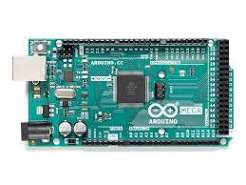
\includegraphics[width=0.2\textwidth]{figures/arduino-mega.png}
    \caption{Carte microcontrôleur Arduino Mega}
\end{figure}

\subsection{ESP32 DEVKIT V1}

Un ESP32 est intégré au système afin d'assurer les fonctions de
communication réseau et l'intégration de la machine dans l'architecture
IoT.

L'ESP32 permet notamment d'établir la communication avec le réseau et de
participer aux échanges de données avec l'infrastructure MQTT.

\begin{figure}[H]
    \centering
    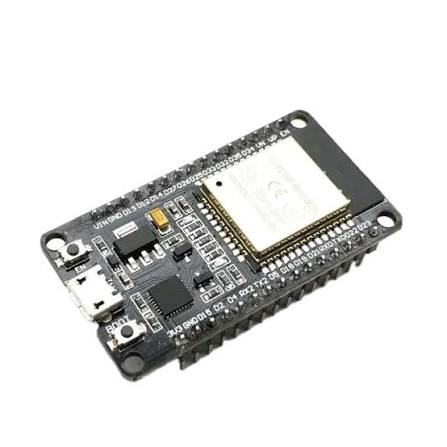
\includegraphics[width=0.18\textwidth]{figures/esp32.png}
    \caption{Carte de développement ESP32 DEVKIT V1}
\end{figure}

\subsection{Moteur pas à pas}

Un moteur pas à pas de type 42BYGH48-23D est utilisé pour assurer
l'entraînement du mécanisme d'extrusion.

Le moteur permet de contrôler précisément le déplacement du mécanisme
grâce à la commande de ses pas.

\begin{figure}[H]
    \centering
    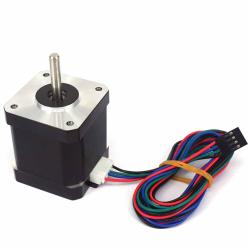
\includegraphics[width=0.2\textwidth]{figures/42bygh48-23d-moteur-pas-a-pas.png}
    \caption{Moteur pas à pas 42BYGH48-23D}
\end{figure}

\subsection{Module moteur pas à pas A4988}

Le moteur pas à pas est commandé à l'aide d'un driver A4988. Celui-ci
permet d'adapter les signaux de commande provenant du microcontrôleur afin
de piloter correctement le moteur.

Le driver permet également d'utiliser différents modes de micro-pas afin
d'améliorer la précision du mouvement.

\begin{figure}[H]
    \centering
    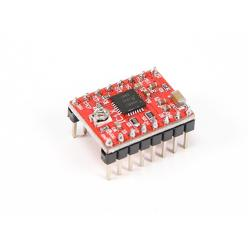
\includegraphics[width=0.2\textwidth]{figures/A4988-driver.png}
    \caption{Driver moteur pas à pas A4988}
\end{figure}

\subsection{Système de chauffage}

Un élément chauffant est utilisé pour chauffer le matériau PET jusqu'à
une température permettant sa transformation et son extrusion.

La température est mesurée à l'aide d'une thermistance et contrôlée par
le système embarqué afin de maintenir une température adaptée au
processus.

\begin{figure}[H]
    \centering
    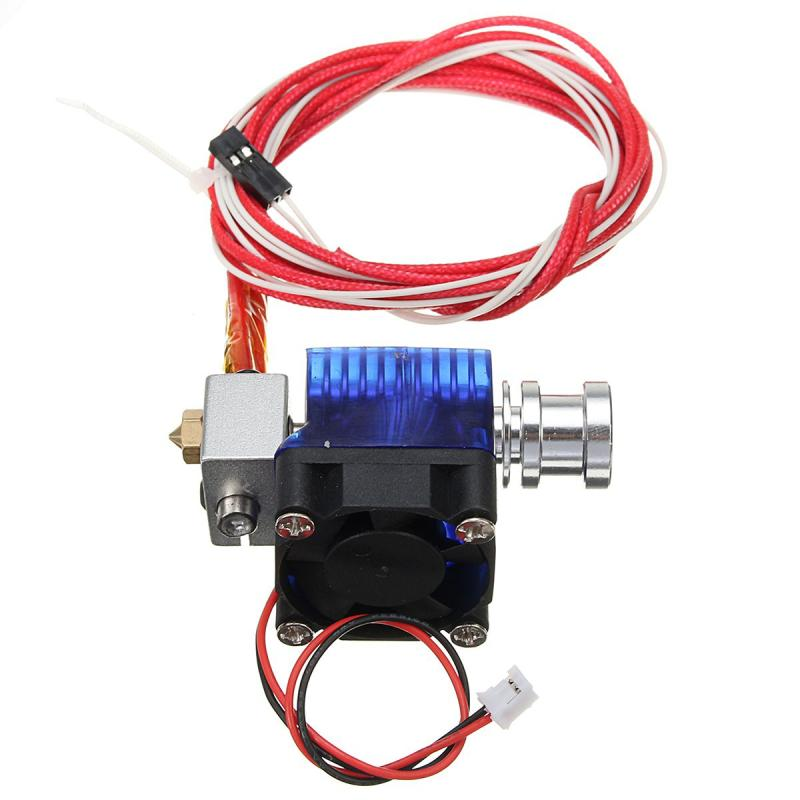
\includegraphics[width=0.23\textwidth]{figures/extrudeuse-simple-tete-17503mm-pour-imprimante-3d-12v.png}
    \caption{Tête d'extrusion chauffante}
\end{figure}

\subsection{Capteur de température}

Une thermistance est utilisée pour mesurer la température du système de
chauffage.

La valeur mesurée est récupérée par le microcontrôleur puis utilisée dans
la boucle de contrôle de température.

\subsection{Module de puissance BTS7960}

Un module de puissance est utilisé pour commander l'élément chauffant à
partir du microcontrôleur.

Cette interface permet de séparer la partie de commande basse tension de
la partie de puissance nécessaire au chauffage.

\begin{figure}[H]
    \centering
    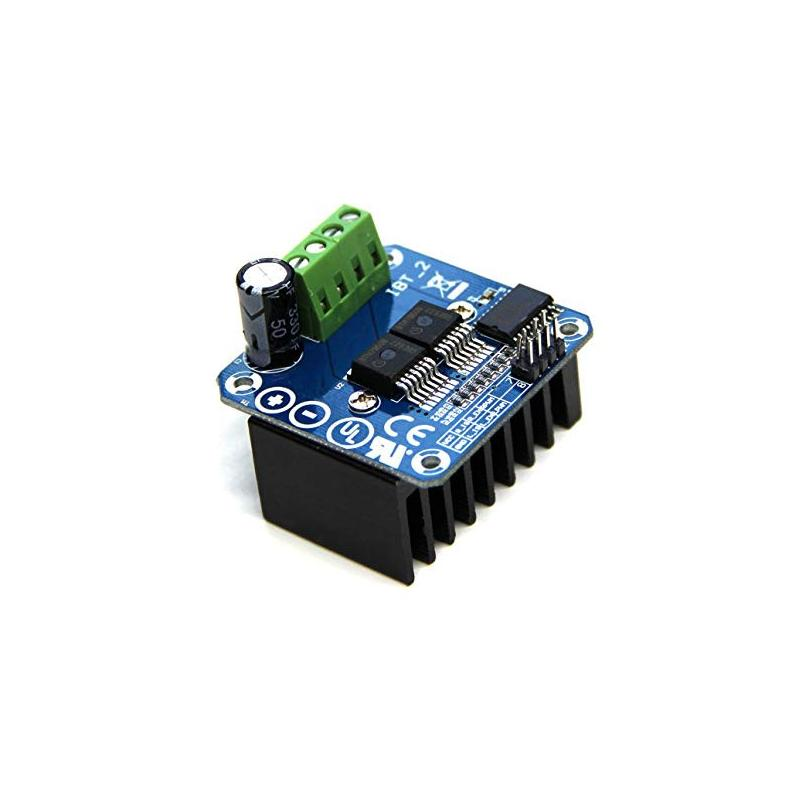
\includegraphics[width=0.2\textwidth]{figures/bts7960.png}
    \caption{Module de puissance BTS7960}
\end{figure}

\subsection{Convertisseur de niveau logique TXS0108}

Un convertisseur de niveau logique est utilisé pour assurer
l'adaptation des niveaux de tension entre les composants fonctionnant sous
différentes tensions logiques.

Cette adaptation est particulièrement importante pour la communication
entre l'Arduino Mega et l'ESP32.

\begin{figure}[H]
    \centering
    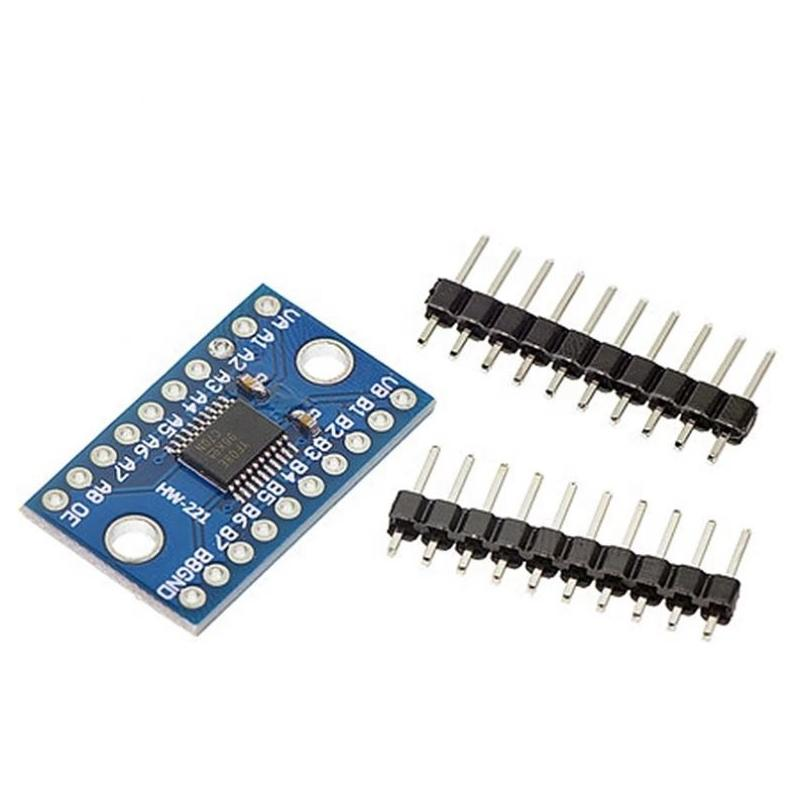
\includegraphics[width=0.2\textwidth]{figures/TXS0108E.png}
    \caption{Convertisseur de niveau logique TXS0108E}
\end{figure}

\subsection{Module convertisseur XL6009E1}
Deux modules convertisseur DC-DC sont utilisés pour fournir les tensions
nécessaires aux microcontrôleurs du système (9v pour l'Arduino Mega et 5v pour l'ESP32).

\begin{figure}[H]
    \centering
    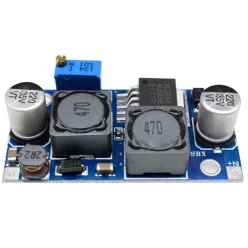
\includegraphics[width=0.2\textwidth]{figures/module-convertisseur-xl6009e.png}
    \caption{Module convertisseur DC-DC XL6009E1}
\end{figure}

\subsection{Alimentation}

La machine utilise une alimentation électrique adaptée aux différents
éléments du système.

Les tensions nécessaires aux composants sont obtenues directement ou à
l'aide de convertisseurs DC-DC afin de fournir des niveaux de tension
appropriés aux circuits électroniques.

\section{Processus du système}

Le fonctionnement général du système peut être décomposé en plusieurs
étapes successives.

\subsection{Préparation du matériau}

Le processus commence par la récupération et la préparation du plastique
PET destiné au recyclage. Le matériau doit être préparé avant son
introduction dans la machine afin de permettre son traitement dans de
bonnes conditions.

\subsection{Mise en température}

Après le démarrage de la machine, le système active le chauffage et mesure
continuellement la température à l'aide de la thermistance.

Le contrôleur compare la température mesurée avec la température de
consigne afin de maintenir les conditions nécessaires à l'extrusion.

\subsection{Extrusion}

Lorsque la température nécessaire est atteinte, le système peut démarrer
le mécanisme d'extrusion.

Le moteur pas à pas entraîne le mécanisme permettant de déplacer le
matériau à travers la zone chauffée. Le PET est ainsi transformé puis
extrudé sous forme de filament.

\subsection{Transmission des données}

Pendant le fonctionnement de la machine, les informations importantes
sont collectées par le système embarqué.

L'Arduino Mega communique avec l'ESP32, qui assure ensuite la transmission
des données vers l'infrastructure IoT.

Les informations peuvent notamment concerner l'état de la machine, la
température et les paramètres associés au processus de production.

\subsection{Supervision}

Les données transmises par la machine sont traitées par le backend puis
mises à disposition des applications web et mobile.

L'utilisateur peut ainsi consulter l'état de la machine et suivre les
informations relatives à son fonctionnement.

\subsection{Fin de production}

À la fin du processus, le système arrête progressivement les éléments
nécessaires au fonctionnement de la machine et enregistre les
informations relatives à la session de production.

Ces données peuvent ensuite être consultées à travers les interfaces de
supervision.

% Insérer ici un schéma du processus global.
%
% \begin{figure}[H]
%     \centering
%     \includegraphics[width=0.9\textwidth]{figures/system-process.png}
%     \caption{Processus global du système}
%     \label{fig:system-process}
% \end{figure}

\section{Interface utilisateur}

L'application \textit{3awedlou} comprend des interfaces permettant à
l'utilisateur de superviser le fonctionnement de la machine et de
consulter les informations disponibles.

Le système comprend une application web ainsi qu'une application mobile.
Les deux interfaces utilisent le même backend afin de centraliser la
gestion des données et des fonctionnalités.

\subsection{Application web}

L'application web constitue une interface de supervision accessible
depuis un navigateur.

Elle permet notamment de consulter les machines disponibles, leur état
actuel ainsi que les informations relatives aux sessions et à la
production.

% Insérer ici les captures de l'application web.
%
% \begin{figure}[H]
%     \centering
%     \includegraphics[width=0.9\textwidth]{figures/web-dashboard.png}
%     \caption{Interface web de supervision}
%     \label{fig:web-dashboard}
% \end{figure}

\subsection{Application mobile}

L'application mobile permet d'accéder aux fonctionnalités principales du
système depuis un smartphone.

Elle reprend les principales fonctions de supervision tout en adaptant
l'organisation des informations à la taille et aux contraintes d'un
écran mobile.

% Insérer ici les captures de l'application mobile.
%
% \begin{figure}[H]
%     \centering
%     \includegraphics[width=0.45\textwidth]{figures/mobile-dashboard.png}
%     \caption{Interface mobile de supervision}
%     \label{fig:mobile-dashboard}
% \end{figure}

\subsection{Communication avec le backend}

Les applications web et mobile communiquent avec le backend afin
d'accéder aux données et aux fonctionnalités du système.

Le backend centralise notamment l'authentification, la gestion des
machines, les données de télémétrie et les informations relatives aux
productions.

Cette architecture permet aux différentes interfaces d'utiliser une
source de données commune tout en conservant une séparation entre la
présentation et la logique métier.

\section{Schéma et câblage}

La réalisation matérielle nécessite l'interconnexion de plusieurs
composants électroniques. Le câblage a été conçu afin de séparer les
différentes fonctions de commande, de puissance, de mesure et de
communication.

L'Arduino Mega assure le contrôle de la partie locale de la machine. Il
est connecté au driver A4988 afin de commander le moteur pas à pas et au
circuit de puissance permettant de piloter le système de chauffage.

La thermistance est connectée à une entrée analogique afin de mesurer la
température du système. Les données de température sont ensuite utilisées
par l'algorithme de contrôle.

L'ESP32 est connecté à l'Arduino Mega afin d'échanger les informations
nécessaires à la communication avec le système IoT. Une adaptation des
niveaux logiques est utilisée pour assurer la compatibilité électrique
entre les deux microcontrôleurs.

L'alimentation électrique est distribuée vers les différents composants
en fonction de leurs tensions et courants nécessaires. Une attention
particulière est portée à la séparation entre les circuits de puissance
et les circuits logiques.

% Insérer ici le schéma électrique complet.
%
% \begin{figure}[H]
%     \centering
%     \includegraphics[width=\textwidth]{figures/schematic-diagram.png}
%     \caption{Schéma électrique du système}
%     \label{fig:schematic}
% \end{figure}

\subsection{Communication Arduino Mega -- ESP32}

La communication entre l'Arduino Mega et l'ESP32 est réalisée à l'aide
d'une liaison série UART.

Cette liaison permet à l'Arduino Mega de transmettre les informations
relatives à l'état de la machine à l'ESP32. Dans le sens inverse, l'ESP32
peut transmettre certaines commandes ou informations nécessaires au
contrôle du système.

La communication série repose sur les lignes TX, RX et GND. Étant donné
que l'Arduino Mega utilise une logique de 5 V alors que l'ESP32 fonctionne
avec une logique de 3,3 V, un convertisseur de niveau logique est utilisé
afin d'assurer une communication compatible avec les deux circuits.

% Insérer ici un schéma simplifié de la liaison UART.
%
% \begin{figure}[H]
%     \centering
%     \includegraphics[width=0.75\textwidth]{figures/uart-communication.png}
%     \caption{Communication UART entre l'Arduino Mega et l'ESP32}
%     \label{fig:uart}
% \end{figure}

\subsection{Commande du moteur}

Le moteur pas à pas est commandé par le driver A4988. L'Arduino Mega
génère les signaux nécessaires à son fonctionnement, notamment les
signaux \textit{STEP} et \textit{DIR}.

Le réglage du driver permet de définir le mode de micro-pas utilisé et
ainsi d'adapter la précision et la vitesse du mouvement aux besoins du
mécanisme d'extrusion.

\subsection{Contrôle de la température}

Le contrôle de la température constitue une fonction importante de la
machine. La thermistance fournit une mesure de la température au
microcontrôleur.

Cette mesure est ensuite utilisée par l'algorithme de régulation afin
d'ajuster la puissance appliquée au système de chauffage et de maintenir
la température autour de la valeur de consigne.

% Insérer ici un schéma du contrôle de température.
%
% \begin{figure}[H]
%     \centering
%     \includegraphics[width=0.85\textwidth]{figures/temperature-control.png}
%     \caption{Principe de contrôle de la température}
%     \label{fig:temperature-control}
% \end{figure}

\section{Conclusion}

Ce chapitre a présenté la réalisation du système \textit{3awedlou}, depuis
les outils de développement et les composants matériels jusqu'à
l'intégration des différents éléments de la solution.

La partie embarquée permet d'assurer le contrôle local de la machine,
tandis que l'ESP32 assure la connectivité nécessaire à son intégration
dans l'architecture IoT. Le backend centralise la gestion des données et
les applications web et mobile permettent leur consultation et leur
supervision.

La réalisation matérielle, le câblage et les différents mécanismes de
communication permettent ainsi de réunir les différentes composantes du
projet au sein d'un système cohérent.

Les résultats obtenus constituent une base permettant de poursuivre les
tests du système, d'améliorer sa fiabilité et d'optimiser le processus de
recyclage et de production du filament.


% =========================================================
% CONCLUSION
% =========================================================

\chapter*{Conclusion générale}

\addcontentsline{toc}{chapter}{Conclusion générale}

Ce projet a permis de concevoir et de réaliser une solution IoT dédiée
au recyclage du plastique PET en filament pour impression 3D.

La réalisation combine une architecture matérielle basée sur des
systèmes embarqués avec une architecture logicielle permettant la
supervision et l'exploitation des données issues de la machine.

Les résultats obtenus constituent une base permettant de poursuivre
l'amélioration du système, notamment au niveau de la fiabilité, de la
communication temps réel et de l'optimisation du processus de recyclage.


% =========================================================
% BIBLIOGRAPHY
% =========================================================

\newpage

\addcontentsline{toc}{chapter}{Bibliographie}

\bibliographystyle{plain}
\bibliography{bibliography/references}


% =========================================================
% END
% =========================================================

\end{document}


% xelatex -interaction=nonstopmode -file-line-error main.tex